\section{Does the model agree with what is known about these enzymes?}
\label{sec:bio-val}

Cross-validation shows that the model generalises within its data-generating process. This section asks three questions that do not share that process: does it recover published specificity it was not shown, does the structural biology of the enzymes agree with what it learned, and does it rank measured kinetics.

\subsection{Recovery of the MMP-9 consensus}
The phage-display consensus of Kridel et al.\ (2001), Pro-Arg-Ser/Thr$\downarrow$Hy-Ser/Thr, was derived from a different experiment and is not in our training data (MEROPS and PICS). Figure~\ref{fig:kcons} overlays it on the learned MMP-9 PSSM. Pro at $\pos{3}$ is the top-ranked residue of twenty ($+\pssmLOPThreePro$ bits), Leu and Ile are the first and second choices at $\prm{1}$ ($\pssmLOPOnePLeu$ and $\pssmLOPOnePIle$), and Arg at $\pos{2}$ is ranked \pssmRankPTwoArg{}\,/\,20 ($\pssmLOPTwoArg$). These are the two features Kridel et al.\ tie to specific enzyme pockets (an S3 subsite that accommodates the bend introduced by Pro, and the deep hydrophobic S1$'$ pocket).

The model does \emph{not} reproduce Ser/Thr at $\pos{1}$ (Thr ranks \pssmRankPOneThr{}\,/\,20, $\pssmLOPOneThr$; Ser is 9th) or at $\prm{2}$ (Ser ranks \pssmRankPTwoPSer{}\,/\,20, Thr \pssmRankPTwoPThr{}\,/\,20). We do not read this as a failure. Kridel et al.\ note that about two thirds of the $\prm{2}$ Thr residues in their selected clones are encoded by the phage vector rather than selected, so the phage consensus over-represents Thr there. At $\pos{1}$ our top residues are Gly, Lys and Arg (\pssmLOPOneGly{}, \pssmLOPOneLys{}, \pssmLOPOneArg{} bits); Gly at $\pos{1}$ is what the natural collagen and other protein substrates in Kridel et al.'s Table~III show (Pro-X-Gly$\downarrow$Hy), and Arg at $\pos{1}$ is favoured in their group~III substrates. The learned specificity is that of natural and proteome-derived sites, which differs from a phage-optimised consensus in exactly the places one would expect.

\begin{figure}[!htbp]
\centering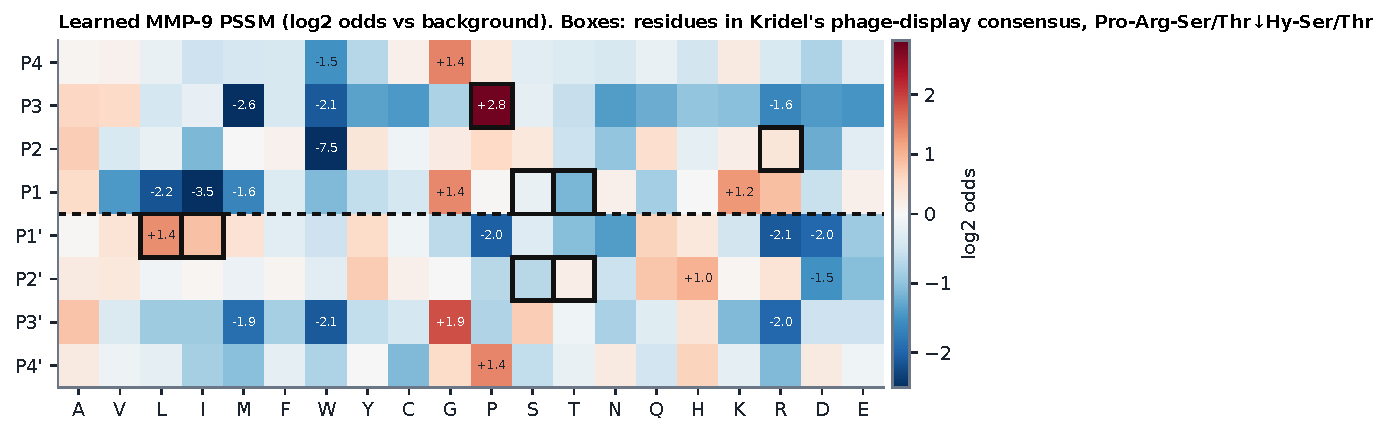
\includegraphics[width=\textwidth]{figures/F14_mmp9_consensus.pdf}
\caption{Learned MMP-9 PSSM (log$_2$ odds against background; only cells with $|{\cdot}|>1$ bit are annotated). Boxes mark the residues of the Kridel et al.\ phage-display consensus. Pro at $\pos{3}$ and Leu/Ile at $\prm{1}$ are recovered; Ser/Thr at $\pos{1}$ and $\prm{2}$ are not (see text).}
\label{fig:kcons}
\end{figure}

\subsection{Learned specificity in the context of the enzyme structures}
\label{sec:structures}
We prepared one experimental structure per protease (Table~\ref{tab:struct}; Figure~\ref{fig:struct}) and derived active-site facts from the coordinates rather than asserting them. In MMP-9, MMP-2 and MMP-8 the sequence around the catalytic zinc reads H-E-F-G-H-A-L-G-L-D/E-H, i.e.\ the HEXXHXXGXXH motif of Nagase and Woessner (1999); the zinc is coordinated by the two histidines of HEXXH and the third histidine of the motif (His401, His405, His411 in MMP-9), and the hydroxamate oxygen of the bound MMP-9 inhibitor lies $2.07$~\AA\ from it. In LasB the zinc ligands are His140, His144 and Glu164; in neutrophil elastase the catalytic triad is His57, Asp102 and Ser195. Residues lining the ligand-occupied pocket of MMP-9 include Asp185-Gly186-Leu187, the Asp-Gly-Leu segment that Kridel et al.\ assign to the S2$'$ subsite (their numbering differs), and Met422. In NE they include Val190, Ala213 and Val216, small aliphatic side chains, and the NE model's top residues at $\pos{1}$ are Val, Ile and Thr (Appendix Table~\ref{tab:topres}).

\begin{table}[!htbp]
\centering\small\begin{tabular}{@{}llcclc@{}}\toprule
Protease & PDB & Resolution (\AA) & Residues & Catalytic site residues & Pocket residues \\\midrule
MMP-2 & 1QIB & 2.8 & 160 & HIS201, HIS205, HIS211 & 23 \\
MMP-8 & 1JAN & 2.5 & 164 & HIS197, HIS201, HIS207 & 21 \\
MMP-9 & 1GKC & 2.3 & 159 & HIS401, HIS405, HIS411 & 20 \\
Neutrophil elastase & 1HNE & 1.84 & 210 & ASP102, HIS57, SER195 & 22 \\
LasB & 1EZM & 1.5 & 298 & GLU164, HIS140, HIS144 & 27 \\
\bottomrule\end{tabular}

\caption{Structures used. The catalytic-site residues are those coordinating the catalytic zinc (MMPs, LasB) or forming the catalytic triad (NE), identified from the coordinates. ``Pocket residues'' are within $6$~\AA\ of the bound ligand, or within $9$~\AA\ of the catalytic zinc when no ligand is present.}
\label{tab:struct}
\end{table}

\begin{figure}[!htbp]
\centering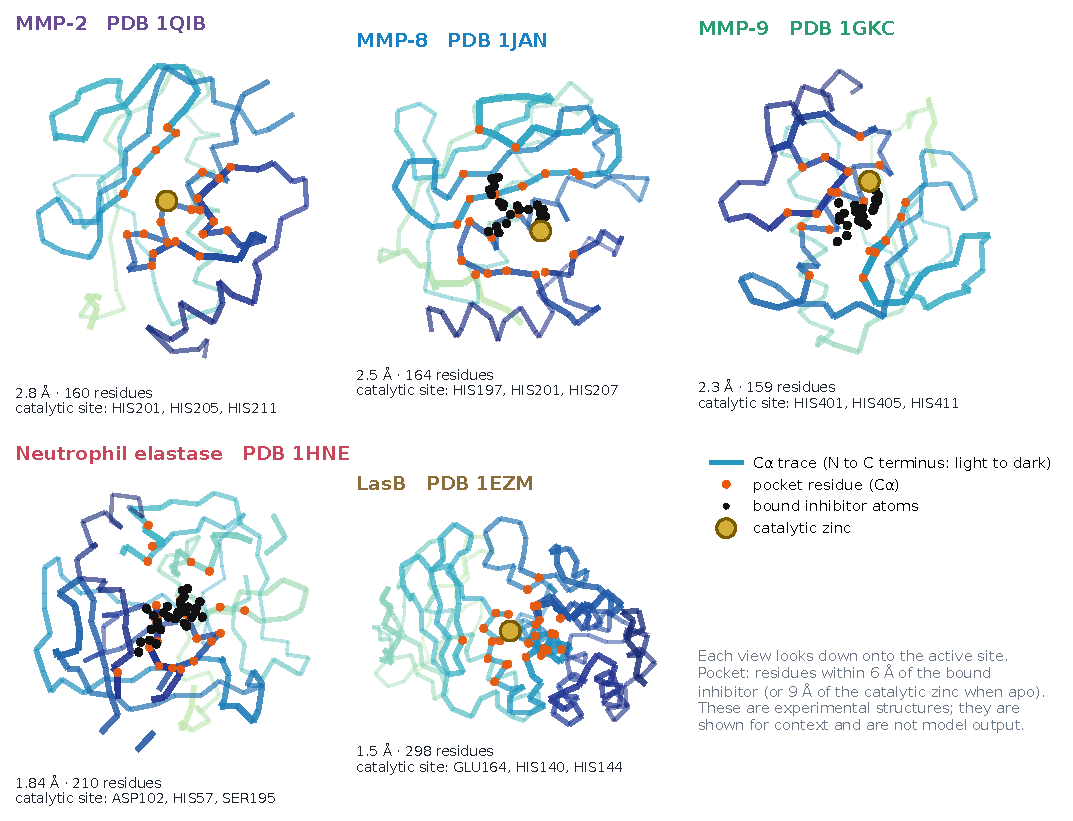
\includegraphics[width=\textwidth]{figures/F19_structures.pdf}
\caption{C$\alpha$ traces of the five structures, each oriented to look at the active site (depth-cued; N to C terminus from light to dark). Orange: pocket residues; gold: catalytic zinc; black: bound inhibitor atoms. These are experimental structures shown for context; they are not model output. MMP-9 is shown from an active catalytic-domain entry, not the pro-form, whose prodomain occupies the cleft.}
\label{fig:struct}
\end{figure}

\subsection{Held-out measured kinetics}
\label{sec:kval}
Kridel et al.\ (2001, their Table~II) measured $\kcat/\Km$ for MMP-9 on eleven synthetic peptides and found no detectable activity on a twelfth (C11). None of these peptides is in the training data after the removal of four coinciding windows (Section~\ref{sec:eval}). We score each as a gapped window (Table~\ref{tab:kscores}) and rank-correlate with $\log_{10}\kcat/\Km$.

\begin{table}[!htbp]
\centering\small\begin{tabular}{@{}llrrrr@{}}\toprule
Peptide & Window (P4--P4$'$) & Positions & MMP-9 $k_\mathrm{cat}/K_m$ (M$^{-1}$s$^{-1}$) & LR logit & PSSM \\\midrule
C15 & \texttt{GPRQITA-} & 7 & 188{,}000 & +2.07 & +5.41 \\
A11 & \texttt{IPRTLTA-} & 7 & 67{,}500 & +1.30 & +3.67 \\
A6 & \texttt{GPRAVSTT} & 8 & 61{,}000 & +1.24 & +4.20 \\
A11m1 & \texttt{IPRRLTA-} & 7 & 160{,}000 & +2.43 & +5.66 \\
A11m2 & \texttt{IPRTATA-} & 7 & 2{,}000 & +1.15 & +2.35 \\
A10 & \texttt{GPLFYSVT} & 8 & 25{,}600 & +0.33 & +2.70 \\
B1 & \texttt{QPHYLTTA} & 8 & 8{,}800 & +0.81 & +3.10 \\
A18 & \texttt{RPAKSTA-} & 7 & 5{,}800 & +1.28 & +4.96 \\
A7 & \texttt{--SGLKAL} & 6 & 12{,}400 & +0.77 & +3.08 \\
A19 & \texttt{GSRYLTA-} & 7 & 13{,}200 & +0.74 & +3.02 \\
A16 & \texttt{SGRRLLSR} & 8 & 1{,}200 & +0.68 & +0.78 \\
C11 & \texttt{SGRRLIHH} & 8 & not detected & +0.30 & +2.47 \\
\bottomrule\end{tabular}

\caption{Validation peptides (Kridel et al., 2001, Table II) as scored P4--P4$'$ windows, with measured MMP-9 $\kcat/\Km$ and model scores from the MMP-9 model retrained without coinciding windows. Positions: number of known positions out of eight.}
\label{tab:kscores}
\end{table}

\begin{table}[!htbp]
\centering\small\begin{tabular}{@{}llccc@{}}\toprule
Score & Set & Spearman $\rho$ & 95\% bootstrap CI & Permutation $p$ \\\midrule
Logistic regression & n = 11 measured & 0.58 & [-0.23, 0.93] & 0.068 \\
Logistic regression & n = 12 (C11 ranked lowest) & 0.68 & [0.02, 0.96] & 0.017 \\
PSSM & n = 11 measured & 0.70 & [-0.00, 0.96] & 0.020 \\
PSSM & n = 12 (C11 ranked lowest) & 0.75 & [0.18, 0.93] & 0.006 \\
Standardised mean & n = 11 measured & 0.57 & [-0.21, 0.90] & 0.074 \\
Standardised mean & n = 12 (C11 ranked lowest) & 0.66 & [0.06, 0.91] & 0.021 \\
\bottomrule\end{tabular}

\caption{Rank association between model score and measured MMP-9 $\kcat/\Km$. The permutation $p$-value is two-sided; intervals are bootstrap over peptides. The last rows include C11 (no activity detected) ranked below every measured peptide.}
\label{tab:kspear}
\end{table}

The association is positive for every scorer and every set (Table~\ref{tab:kspear}; Figure~\ref{fig:kval}). For the PSSM it is $\rho=\rhoNElevenPSSM$ on the eleven measured peptides (permutation $p=\rhoPNElevenPSSM$; $95\%$ interval $[\rhoLoNElevenPSSM,\rhoHiNElevenPSSM]$); for the logistic regression $\rho=\rhoNElevenLR$ ($p=\rhoPNElevenLR$). The intervals are wide and, for the logistic regression on $n=11$, include zero. With $n=11$ and a set that was itself selected for high activity, this is evidence of a positive association, not of accurate rate prediction, and the six tests are not corrected for multiplicity. By the logistic regression the three highest-scored peptides (A11m1, C15, A11) are the three most active; its largest miss is A10 ($25{,}600$~M$^{-1}$s$^{-1}$, the fifth most active), which it scores second-lowest. The PSSM scores the least active measured peptide (A16) lowest, but ranks A18 ($5{,}800$) third, its largest miss.

\begin{figure}[!htbp]
\centering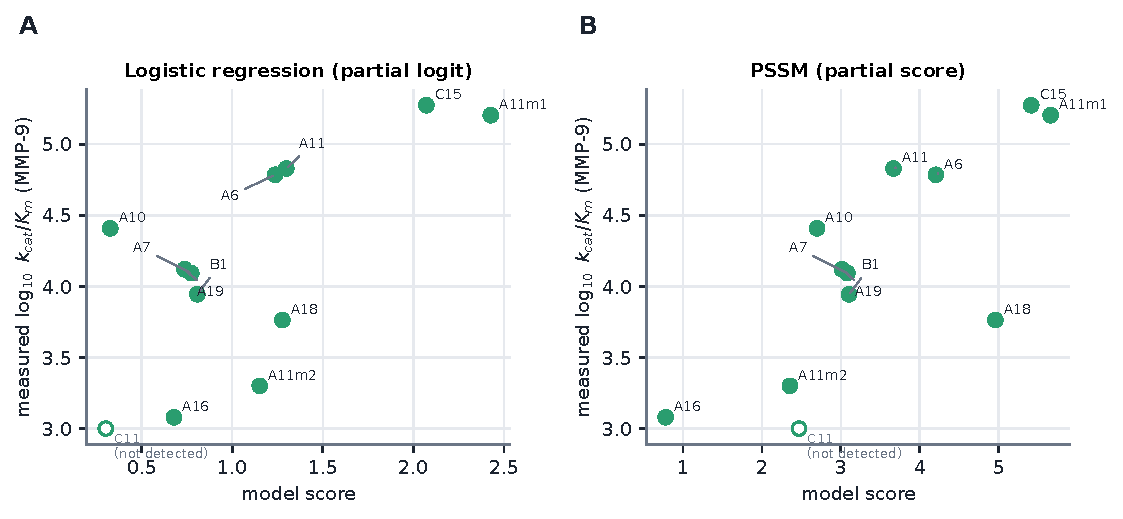
\includegraphics[width=\textwidth]{figures/F15_kridel_validation.pdf}
\caption{Model score against measured MMP-9 $\log_{10}\kcat/\Km$. Open marker: C11, no activity detected (plotted at the floor of the axis).}
\label{fig:kval}
\end{figure}

\subsubsection{Matched point mutants}
Two peptides are single-substitution mutants of A11 (SGKIPRT$\downarrow$LTA): A11m1 replaces Thr with Arg at $\pos{1}$; A11m2 replaces Leu with Ala at $\prm{1}$. Because the background is identical, they isolate one substitution each (Table~\ref{tab:kmut}). The model predicts the correct direction for both and roughly the correct size for the first ($+\mutOneLR$ bits from the logistic regression and $+\mutOnePSSM$ from the PSSM against a measured $+\mutOneMeasured$~log$_2$ units). For the second it predicts a decrease but underestimates it badly: $\mutTwoLR$ bits (logistic regression) and $\mutTwoPSSM$ bits (PSSM) against a measured $\mutTwoMeasured$. Large kinetic effects of a single key residue are compressed by a model trained to distinguish cleaved from uncleaved sites rather than fast from slow.

\begin{table}[!htbp]
\centering\small\begin{tabular}{@{}llccc@{}}\toprule
Pair & Substitution & Measured fold change (log$_2$) & LR $\Delta$ (bits) & PSSM $\Delta$ (bits) \\\midrule
A11$\to$A11m1 & T7R at P1 (Thr to Arg) & 2.37$\times$ (+1.25) & +1.63 & +1.99 \\
A11$\to$A11m2 & L8A at P1' (Leu to Ala) & 0.03$\times$ (-5.08) & -0.21 & -1.31 \\
\bottomrule\end{tabular}

\caption{Model change in score for the two matched mutants of A11, compared with the measured change in $\kcat/\Km$.}
\label{tab:kmut}
\end{table}
